%  LaTeX support: latex@mdpi.com 
%  For support, please attach all files needed for compiling as well as the log file, and specify your operating system, LaTeX version, and LaTeX editor.

%=================================================================
\documentclass[entropy,article,submit,pdftex,moreauthors]{Definitions/mdpi} 
%\documentclass[preprints,article,submit,pdftex,moreauthors]{Definitions/mdpi} 
% For posting an early version of this manuscript as a preprint, you may use "preprints" as the journal. Changing "submit" to "accept" before posting will remove line numbers.

% Below journals will use APA reference format:
% admsci, aieduc, behavsci, businesses, econometrics, economies, education, ejihpe, famsci, games, humans, ijcs, ijfs, journalmedia, jrfm, languages, psycholint, publications, tourismhosp, youth

% Below journals will use Chicago reference format:
% arts, genealogy, histories, humanities, jintelligence, laws, literature, religions, risks, socsci

%--------------------
% Class Options:
%--------------------
%----------
% journal
%----------
% Choose between the following MDPI journals:
% accountaudit, acoustics, actuators, addictions, adhesives, admsci, adolescents, aerobiology, aerospace, agriculture, agriengineering, agrochemicals, agronomy, ai, air, algorithms, allergies, alloys, amh, analytica, analytics, anatomia, anesthres, animals, antibiotics, antibodies, antioxidants, applbiosci, appliedchem, appliedmath, appliedphys, applmech, applmicrobiol, applnano, applsci, aquacj, architecture, arm, arthropoda, arts, asc, asi, astronomy, atmosphere, atoms, audiolres, automation, axioms, bacteria, batteries, bdcc, behavsci, beverages, biochem, bioengineering, biologics, biology, biomass, biomechanics, biomed, biomedicines, biomedinformatics, biomimetics, biomolecules, biophysica, biosensors, biosphere, biotech, birds, blockchains, bloods, blsf, brainsci, breath, buildings, businesses, cancers, carbon, cardiogenetics, catalysts, cells, ceramics, challenges, chemengineering, chemistry, chemosensors, chemproc, children, chips, cimb, civileng, cleantechnol, climate, clinbioenerg, clinpract, clockssleep, cmd, cmtr, coasts, coatings, colloids, colorants, commodities, complications, compounds, computation, computers, condensedmatter, conservation, constrmater, cosmetics, covid, crops, cryo, cryptography, crystals, csmf, ctn, curroncol, cyber, dairy, data, ddc, dentistry, dermato, dermatopathology, designs, devices, diabetology, diagnostics, dietetics, digital, disabilities, diseases, diversity, dna, drones, dynamics, earth, ebj, ecm, ecologies, econometrics, economies, education, eesp, ejihpe, electricity, electrochem, electronicmat, electronics, encyclopedia, endocrines, energies, eng, engproc, ent, entomology, entropy, environments, epidemiologia, epigenomes, esa, est, famsci, fermentation, fibers, fintech, fire, fishes, fluids, foods, forecasting, forensicsci, forests, fossstud, foundations, fractalfract, fuels, future, futureinternet, futureparasites, futurepharmacol, futurephys, futuretransp, galaxies, games, gases, gastroent, gastrointestdisord, gastronomy, gels, genealogy, genes, geographies, geohazards, geomatics, geometry, geosciences, geotechnics, geriatrics, glacies, grasses, greenhealth, gucdd, hardware, hazardousmatters, healthcare, hearts, hemato, hematolrep, heritage, higheredu, highthroughput, histories, horticulturae, hospitals, humanities, humans, hydrobiology, hydrogen, hydrology, hygiene, idr, iic, ijerph, ijfs, ijgi, ijmd, ijms, ijns, ijpb, ijt, ijtm, ijtpp, ime, immuno, informatics, information, infrastructures, inorganics, insects, instruments, inventions, iot, j, jal, jcdd, jcm, jcp, jcs, jcto, jdad, jdb, jeta, jfb, jfmk, jimaging, jintelligence, jlpea, jmahp, jmmp, jmms, jmp, jmse, jne, jnt, jof, joitmc, joma, jop, jor, journalmedia, jox, jpbi, jpm, jrfm, jsan, jtaer, jvd, jzbg, kidney, kidneydial, kinasesphosphatases, knowledge, labmed, laboratories, land, languages, laws, life, lights, limnolrev, lipidology, liquids, literature, livers, logics, logistics, lubricants, lymphatics, machines, macromol, magnetism, magnetochemistry, make, marinedrugs, materials, materproc, mathematics, mca, measurements, medicina, medicines, medsci, membranes, merits, metabolites, metals, meteorology, methane, metrics, metrology, micro, microarrays, microbiolres, microelectronics, micromachines, microorganisms, microplastics, microwave, minerals, mining, mmphys, modelling, molbank, molecules, mps, msf, mti, multimedia, muscles, nanoenergyadv, nanomanufacturing, nanomaterials, ncrna, ndt, network, neuroglia, neurolint, neurosci, nitrogen, notspecified, nursrep, nutraceuticals, nutrients, obesities, oceans, ohbm, onco, oncopathology, optics, oral, organics, organoids, osteology, oxygen, parasites, parasitologia, particles, pathogens, pathophysiology, pediatrrep, pets, pharmaceuticals, pharmaceutics, pharmacoepidemiology, pharmacy, philosophies, photochem, photonics, phycology, physchem, physics, physiologia, plants, plasma, platforms, pollutants, polymers, polysaccharides, populations, poultry, powders, preprints, proceedings, processes, prosthesis, proteomes, psf, psych, psychiatryint, psychoactives, psycholint, publications, purification, quantumrep, quaternary, qubs, radiation, reactions, realestate, receptors, recycling, regeneration, religions, remotesensing, reports, reprodmed, resources, rheumato, risks, robotics, rsee, ruminants, safety, sci, scipharm, sclerosis, seeds, sensors, separations, sexes, signals, sinusitis, siuj, skins, smartcities, sna, societies, socsci, software, soilsystems, solar, solids, spectroscj, sports, standards, stats, std, stresses, surfaces, surgeries, suschem, sustainability, symmetry, synbio, systems, tae, targets, taxonomy, technologies, telecom, test, textiles, thalassrep, therapeutics, thermo, timespace, tomography, tourismhosp, toxics, toxins, transplantology, transportation, traumacare, traumas, tropicalmed, universe, urbansci, uro, vaccines, vehicles, venereology, vetsci, vibration, virtualworlds, viruses, vision, waste, water, wem, wevj, wild, wind, women, world, youth, zoonoticdis

%---------
% article
%---------
% The default type of manuscript is "article", but can be replaced by: 
% abstract, addendum, article, benchmark, book, bookreview, briefcommunication, briefreport, casereport, changes, clinicopathologicalchallenge, comment, commentary, communication, conceptpaper, conferenceproceedings, correction, conferencereport, creative, datadescriptor, discussion, entry, expressionofconcern, extendedabstract, editorial, essay, erratum, fieldguide, hypothesis, interestingimages, letter, meetingreport, monograph, newbookreceived, obituary, opinion, proceedingpaper, projectreport, reply, retraction, review, perspective, protocol, shortnote, studyprotocol, supfile, systematicreview, technicalnote, viewpoint, guidelines, registeredreport, tutorial,  giantsinurology, urologyaroundtheworld
% supfile = supplementary materials

%----------
% submit
%----------
% The class option "submit" will be changed to "accept" by the Editorial Office when the paper is accepted. This will only make changes to the frontpage (e.g., the logo of the journal will get visible), the headings, and the copyright information. Also, line numbering will be removed. Journal info and pagination for accepted papers will also be assigned by the Editorial Office.

%------------------
% moreauthors
%------------------
% If there is only one author the class option oneauthor should be used. Otherwise use the class option moreauthors.

%---------
% pdftex
%---------
% The option pdftex is for use with pdfLaTeX. Remove "pdftex" for (1) compiling with LaTeX & dvi2pdf (if eps figures are used) or for (2) compiling with XeLaTeX.

%=================================================================
% MDPI internal commands - do not modify
\firstpage{1} 
\makeatletter 
\setcounter{page}{\@firstpage} 
\makeatother
\pubvolume{1}
\issuenum{1}
\articlenumber{0}
\pubyear{2025}
\copyrightyear{2025}
%\externaleditor{Firstname Lastname} % More than 1 editor, please add `` and '' before the last editor name
\datereceived{ } 
\daterevised{ } % Comment out if no revised date
\dateaccepted{ } 
\datepublished{ } 
%\datecorrected{} % For corrected papers: "Corrected: XXX" date in the original paper.
%\dateretracted{} % For retracted papers: "Retracted: XXX" date in the original paper.
\hreflink{https://doi.org/} % If needed use \linebreak
%\doinum{}
%\pdfoutput=1 % Uncommented for upload to arXiv.org
%\CorrStatement{yes}  % For updates
%\longauthorlist{yes} % For many authors that exceed the left citation part

%=================================================================
% Add packages and commands here. The following packages are loaded in our class file: fontenc, inputenc, calc, indentfirst, fancyhdr, graphicx, epstopdf, lastpage, ifthen, float, amsmath, amssymb, lineno, setspace, enumitem, mathpazo, booktabs, titlesec, etoolbox, tabto, xcolor, colortbl, soul, multirow, microtype, tikz, totcount, changepage, attrib, upgreek, array, tabularx, pbox, ragged2e, tocloft, marginnote, marginfix, enotez, amsthm, natbib, hyperref, cleveref, scrextend, url, geometry, newfloat, caption, draftwatermark, seqsplit
% cleveref: load \crefname definitions after \begin{document}
%\usepackage{subfigure}
\usepackage{subcaption}
\usepackage{tikz}
\usetikzlibrary{angles, quotes}
\usepackage{pgfplots}
\pgfplotsset{compat=1.17}
%=================================================================
% Please use the following mathematics environments: Theorem, Lemma, Corollary, Proposition, Characterization, Property, Problem, Example, ExamplesandDefinitions, Hypothesis, Remark, Definition, Notation, Assumption
%% For proofs, please use the proof environment (the amsthm package is loaded by the MDPI class).

%=================================================================
% Full title of the paper (Capitalized)
\Title{Time Dilation from Quantum Substrate Dynamics: A Coherence-Based Origin for Relativistic Delay}

% MDPI internal command: Title for citation in the left column
\TitleCitation{Title}

% Author Orchid ID: enter ID or remove command
\newcommand{\orcidauthorA}{0009-0003-9747-9109} % Add \orcidA{} behind the author's name
%\newcommand{\orcidauthorB}{0000-0000-0000-000X} % Add \orcidB{} behind the author's name

% Authors, for the paper (add full first names)
\Author{Michael Bush $^{1}$\orcidA{}}

%\longauthorlist{yes}

% MDPI internal command: Authors, for metadata in PDF
\AuthorNames{Michael Bush}

% MDPI internal command: Authors, for citation in the left column, only choose below one of them according to the journal style
% If this is a Chicago style journal 
% (arts, genealogy, histories, humanities, jintelligence, laws, literature, religions, risks, socsci): 
% Lastname, Firstname, Firstname Lastname, and Firstname Lastname.

% If this is a APA style journal 
% (admsci, behavsci, businesses, econometrics, economies, education, ejihpe, games, humans, ijfs, journalmedia, jrfm, languages, psycholint, publications, tourismhosp, youth): 
% Lastname, F., Lastname, F., \& Lastname, F.

% If this is a ACS style journal (Except for the above Chicago and APA journals, all others are in the ACS format): 
% Lastname, F.; Lastname, F.; Lastname, F.
\isAPAStyle{%
       \AuthorCitation{Lastname, F., Lastname, F., \& Lastname, F.}
         }{%
        \isChicagoStyle{%
        \AuthorCitation{Lastname, Firstname, Firstname Lastname, and Firstname Lastname.}
        }{
        \AuthorCitation{Lastname, F.; Lastname, F.; Lastname, F.}
        }
}

% Affiliations / Addresses (Add [1] after \address if there is only one affiliation.)
\address{%
$^{1}$ \quad Hadden Technologies Corporation; mbush@haddentechnologies.com\\
%$^{2}$ \quad Affiliation 2; e-mail@e-mail.com
}

% Contact information of the corresponding author
\corres{Correspondence: mbush@haddentechnologies.com (M.B.)}

% Current address and/or shared authorship
%\firstnote{Shiloh, IL: Independent Researcher.}  % Current address should not be the same as any items in the Affiliation section.
%\secondnote{These authors contributed equally to this work.}
% The commands \thirdnote{} till \eighthnote{} are available for further notes

%\simplesumm{} % Simple summary

%\conference{} % An extended version of a conference paper


% Abstract (Do not insert blank lines, i.e. \\) 
\abstract{Time dilation is a well-established relativistic effect, yet its physical origin remains undefined within traditional geometric frameworks. In this work, we derive time dilation from first principles using the Quantum Substrate Dynamics (QSD) model, where time emerges as a quantized delay associated with local phase coherence recovery. In this view, each region of space is characterized by a coherence support length \texorpdfstring{\( L_{\text{coh}} \)}, and time flows at a rate determined by the scalar recovery speed \texorpdfstring{\( c_s \)}:
\texorpdfstring{\[
\tau(x) = \frac{L_{\text{coh}}(x)}{c_s}
\]}\\
Gravitational dilation arises from stretch in the coherence field near a mass-phase, while kinematic effects emerge from projection of motion into the substrate's scalar recovery bandwidth. Together, these mechanisms yield a unified expression for time dilation without reference to coordinate transformations or invariant light speed.
The resulting equation matches observed effects—including GPS clock offsets and muon lifetime extension—using only physically interpretable substrate terms. This approach replaces abstract geometry with a conserved coherence field, providing the first axiom-free, mechanical explanation of relativistic time delay. In doing so, QSD reframes time as a dynamic, field-based phenomenon grounded in substrate deformation rather than observation.}

% Keywords
\keyword{Quantum Substrate Dynamics; coherence recovery; time dilation; causal conservation; scalar tick; relativistic delay; phase drag; substrate saturation; Lorentz factor derivation} 

% The fields PACS, MSC, and JEL may be left empty or commented out if not applicable
%\PACS{J0101}
%\MSC{}
%\JEL{}

%%%%%%%%%%%%%%%%%%%%%%%%%%%%%%%%%%%%%%%%%%
% Only for the journal Diversity
%\LSID{\url{http://}}

%%%%%%%%%%%%%%%%%%%%%%%%%%%%%%%%%%%%%%%%%%
% Only for the journal Applied Sciences
%\featuredapplication{Authors are encouraged to provide a concise description of the specific application or a potential application of the work. This section is not mandatory.}
%%%%%%%%%%%%%%%%%%%%%%%%%%%%%%%%%%%%%%%%%%

%%%%%%%%%%%%%%%%%%%%%%%%%%%%%%%%%%%%%%%%%%
% Only for the journal Data
%\dataset{DOI number or link to the deposited data set if the data set is published separately. If the data set shall be published as a supplement to this paper, this field will be filled by the journal editors. In this case, please submit the data set as a supplement.}
%\datasetlicense{License under which the data set is made available (CC0, CC-BY, CC-BY-SA, CC-BY-NC, etc.)}

%%%%%%%%%%%%%%%%%%%%%%%%%%%%%%%%%%%%%%%%%%
% Only for the journal BioTech, Fishes, Neuroimaging and Toxins
%\keycontribution{The breakthroughs or highlights of the manuscript. Authors can write one or two sentences to describe the most important part of the paper.}

%%%%%%%%%%%%%%%%%%%%%%%%%%%%%%%%%%%%%%%%%%
% Only for the journal Encyclopedia
%\encyclopediadef{For entry manuscripts only: please provide a brief overview of the entry title instead of an abstract.}

%%%%%%%%%%%%%%%%%%%%%%%%%%%%%%%%%%%%%%%%%%
% Only for the journal Advances in Respiratory Medicine, Future, Sensors and Smart Cities
%\addhighlights{yes}
%\renewcommand{\addhighlights}{%
%
%\noindent This is an obligatory section in ``Advances in Respiratory Medicine'', ``Future'', ``Sensors'' and ``Smart Cities”, whose goal is to increase the discoverability and readability of the article via search engines and other scholars. Highlights should not be a copy of the abstract, but a simple text allowing the reader to quickly and simplified find out what the article is about and what can be cited from it. Each of these parts should be devoted up to 2~bullet points.\vspace{3pt}\\
%\textbf{What are the main findings?}
% \begin{itemize}[labelsep=2.5mm,topsep=-3pt]
% \item First bullet.
% \item Second bullet.
% \end{itemize}\vspace{3pt}
%\textbf{What is the implication of the main finding?}
% \begin{itemize}[labelsep=2.5mm,topsep=-3pt]
% \item First bullet.
% \item Second bullet.
% \end{itemize}
%}

%%%%%%%%%%%%%%%%%%%%%%%%%%%%%%%%%%%%%%%%%%
\begin{document}

%%%%%%%%%%%%%%%%%%%%%%%%%%%%%%%%%%%%%%%%%%


% The order of the section titles is different for some journals. Please refer to the "Instructions for Authors” on the journal homepage.

\section{Introduction}

Time dilation is one of the most well-known predictions of modern physics, traditionally interpreted as a consequence of Lorentz invariance and spacetime geometry. From the earliest formulations of the Lorentz transformation to Einstein’s postulates of special\cite{einstein1905} and general relativity \cite{einstein1915}, the slowing of time due to velocity or gravitational potential has been embedded into the mathematical structure of coordinate systems and metric curvature. Despite its experimental confirmation—such as through the Global Positioning System (GPS)~\cite{ashby-gps} and relativistic muon lifetime extension~\cite{bailey-muon}—the physical origin of time dilation remains undefined. The phenomenon is typically accepted as a geometric artifact rather than a causally derived result.

In this work, we present a first-principles derivation of time dilation using the framework of Quantum Substrate Dynamics (QSD)~\cite{bush2025}. QSD is a Lorentz-invariant, coherence-based field theory in which time, mass, and quantization emerge from causal interactions within a conserved physical substrate. This substrate supports two orthogonal propagation modes: a scalar coherence recovery velocity \( c_s \), which governs phase restoration pacing, and a transverse coherence spread velocity \( c_t \), which determines spatial coherence support geometry. In this framework, time is not an abstract coordinate axis, but the interval required for local substrate recovery following energy offload~\cite{bush-planck-2025}. This approach follows the same structural logic used to derive Planck’s constant in prior work, where \( \hbar \) was shown to arise from the ratio of transverse to scalar coherence dynamics. That result established the substrate’s role in setting quantization thresholds; here, we apply those principles to the pacing behavior that defines time.

In QSD, this interval is expressed as \( \tau(x) = \frac{L_{\text{coh}}(x)}{c_s} \), where \( \tau(x) \) represents the delay between causal recovery cycles at a given point in space. Time dilation in this context refers to an increase in that delay—i.e., a longer tick interval—rather than an abstract transformation of coordinate rate. When comparing to conventional relativistic results, where faster clocks are observed at altitude or under motion, one must interpret such effects as inverses of the QSD-defined interval: greater tick rate corresponds to smaller \( \tau \).

We show that motion and gravitational fields alter the coherence configuration of the substrate, reducing the available scalar recovery bandwidth and stretching the coherence support length. This deformation leads directly to a unified expression for time dilation—matching experimental results without requiring coordinate transformations or fitted constants. The result complements previous QSD derivations, including the structural origin of Planck’s constant, by extending the same substrate-based dynamics to relativistic timing phenomena.




%%%%%%%%%%%%%%%%%%%%%%%%%%%%%%%%%%%%%%%%%%
\section{Materials and Methods}

This manuscript was developed through a combination of theoretical derivation, conservation-based modeling, and coherence-structured synthesis. The time dilation equation was formulated by the author using first-principles substrate dynamics, with all mathematical expressions derived to maintain causal consistency, empirical validity, and structural compatibility with known relativistic behavior.

In support of the editorial process, generative AI tools—specifically OpenAI's ChatGPT (version GPT-4o, 2025)—were used to assist in:
\begin{itemize}
    \item Generating illustrative figures based on the author’s conceptual framework, with iterative refinement to ensure fidelity to the substrate-based dynamics of the model,
    \item Researching, validating, and cross-referencing related scientific concepts to improve accuracy, contextual alignment, and clarity,
    \item Summarizing and formatting externally sourced material already selected by the author.
\end{itemize}

No original theoretical contributions were generated by the AI system; all scientific claims, hypotheses, derivations, and interpretations were authored and reviewed by the human researcher. The use of ChatGPT is disclosed in alignment with journal policy for transparency in the writing process.

%%%%%%%%%%%%%%%%%%%%%%%%%%%%%%%%%%%%%%%%%%
%\section{Results}

%%%%%%%%%%%%%%%%%%%%%%%%%%%%%%%%%%%%%%%%%%
\section{Discussion}

\subsection{Time as Recovery Delay in a Conserved Substrate}

In the QSD framework, time is not a coordinate, metric interval, or background structure. It is defined physically as the delay required for the substrate to recover local coherence after a quantized offload event. This approach shifts the notion of time from an abstract axis to a mechanical, causal process grounded in phase conservation.

When a system is at rest, scalar recovery occurs at the substrate’s natural rate \( c_s \), pacing the local tick interval. When the system moves relative to the substrate, a portion of its causal bandwidth is redirected to maintain transverse coherence along the motion vector. This projection reduces the available capacity for scalar recovery. The resulting delay is not imposed by geometric deformation but emerges from competition between motion and recovery within a conserved causal structure.

This mechanism reinterprets time dilation not as a coordinate transformation, but as a field-induced conservation response. The scalar tick stretches because the substrate cannot recover fast enough to maintain phase continuity without sacrificing timing resolution. This approach preserves Lorentz invariance without invoking geometry.

\subsection{Gradient Effects and the Stretching of Coherence Support}

In addition to motion-induced delay, QSD predicts that gravitational dilation arises from geometric deformation of the coherence zone. As a system enters a region of reduced gravitational curvature, the substrate's transverse coherence zone expands in response to the diminished field tension. The coherence area \( L_{\text{coh}}(r)^2 \) expands, increasing the scalar recovery path and thus the duration of each tick.

Importantly, this effect is not due to gravitational ``time warping'' but to a real change in substrate geometry required to maintain coherence across a curved field. The result is an increase in scalar delay that mirrors gravitational redshift. The final form of the time dilation equation fuses both of these contributions—projected motion tension and geometric support distortion—into a unified, conservation-respecting expression.

\subsection{Directionality and the Limits of Substrate Response}

An essential feature of the QSD model is its treatment of directionality. Time dilation does not occur uniformly in all directions, but emerges specifically from the projection of motion or curvature into the scalar recovery axis. When the motion vector \( \vec{v} \) aligns with the substrate’s transverse mode \( \vec{c_t} \), scalar recovery must delay to preserve coherence. The effective tick rate is then governed by the remaining projection onto the scalar axis \( \vec{c_s} \), forming the basis of the coherence triangle, Figure \ref{fig:coherence-triangle}.

\begin{figure}[ht]
\centering
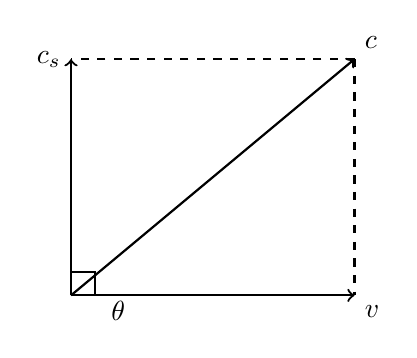
\begin{tikzpicture}[scale=2, thick]

% Triangle sides
\draw[->] (0,0) -- (1.8,0) node[below right] {$v$};
\draw[->] (0,0) -- (0,1.5) node[left] {$c_s$};
\draw[->] (0,0) -- (1.8,1.5) node[above right] {$c$};

% Dotted projections
\draw[dashed] (1.8,1.5) -- (1.8,0);
\draw[dashed] (1.8,1.5) -- (0,1.5);

% Right angle marker
\draw (0.15,0) -- (0.15,0.15) -- (0,0.15);

% Angle labels (optional)
\draw (0.3,0.03) node[below] {$\theta$};

% Label caption
\end{tikzpicture}
\caption{Projection geometry in QSD. The speed of light \( c \) defines the coherence vector, decomposed into scalar recovery \( c_s \) and velocity \( v \) components. Motion through the substrate reduces scalar recovery capacity via projection, giving rise to Lorentz-like time dilation.}
\label{fig:coherence-triangle}
\end{figure}

As velocity approaches the causal limit \( c_s \), this projection collapses, and scalar recovery halts. This reproduces the observed asymptotic freezing of time at relativistic speeds as a consequence of substrate saturation, Figure \ref{fig:relativistic-triangle}. Gradient effects behave similarly: in strong curvature, the substrate must stretch to span distorted regions, increasing recovery delay. However, at extreme velocities, motion dominates, and gradient effects are suppressed—revealing a natural hierarchy of dilation influences.

\begin{figure}[ht]
\centering
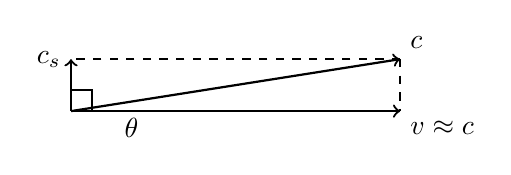
\begin{tikzpicture}[scale=2.2, thick]

% Base line (v)
\draw[->] (0,0) -- (1.9,0) node[below right] {$v \approx c$};

% Scalar recovery (c_s) – very short
\draw[->] (0,0) -- (0,0.3) node[left] {$c_s$};

% Coherence vector c (hypotenuse)
\draw[->] (0,0) -- (1.9,0.3) node[above right] {$c$};

% Dotted projections
\draw[dashed] (1.9,0.3) -- (1.9,0);
\draw[dashed] (1.9,0.3) -- (0,0.3);

% Right angle marker
\draw (0.12,0) -- (0.12,0.12) -- (0,0.12);

% Optional: angle label
\node[below right] at (0.25,0.02) {$\theta$};

\end{tikzpicture}
\caption{In the relativistic regime, motion approaches the total coherence budget \( c \), reducing scalar recovery \( c_s \) to near zero. The substrate’s ability to recover local coherence is saturated by motion, leading to extreme time dilation.}
\label{fig:relativistic-triangle}
\end{figure}

%%%%%%%%%%%%%%%%%%%%%%%%%%%%%%%%%%%%%%%%%%%%%%%%%%%%%
%%%%%%%%%%%%%%%%%%%%%%%%%%%%%%%%%%%%%%%%%%%%%%%%%%%%%

\subsection{Structural Derivation of the Time Dilation Equation}

In Quantum Substrate Dynamics (QSD), all physical phenomena—including time—emerge from causal interactions within a conserved, deformable coherence substrate. This substrate supports two orthogonal propagation modes:

\begin{itemize}
  \item \textbf{Scalar mode} \( c_s \): governs longitudinal phase recovery (timing) after energy offload,
  \item \textbf{Transverse mode} \( c_t \): governs lateral coherence spread across spatial regions.
\end{itemize}

Time is not defined as a coordinate or metric interval, but as the physical delay required for the substrate to restore local coherence. When a system undergoes a quantized energy offload, the substrate must phase-stabilize the region. The time associated with this stabilization is the local tick interval:
\begin{equation}
\tau(x) = \frac{L_{\text{coh}}(x)}{c_s},
\end{equation}
where \( L_{\text{coh}}(x) \) is the local coherence support length and \( c_s \) is the scalar recovery velocity. This definition makes time a field-dependent pacing delay rather than an abstract axis.

\subsubsection{Motion-Induced Scalar Recovery Delay}

Motion through the substrate redirects part of the causal recovery capacity toward maintaining transverse coherence continuity. This effect can be modeled by a coherence projection triangle:
\begin{equation}
c^2 = c_s^2 + v^2,
\end{equation}
which yields the reduced scalar recovery velocity:
\begin{equation}
c_s = \sqrt{c^2 - v^2}.
\end{equation}
The local delay associated with motion is then:
\begin{equation}
\tau_{\text{motion}} = \frac{L_{\text{coh}}}{\sqrt{c^2 - v^2}} = \frac{L_{\text{coh}}}{c_s} \cdot \frac{1}{\sqrt{1 - \frac{v^2}{c^2}}}.
\end{equation}
This reproduces the Lorentz factor, but now as a consequence of finite scalar bandwidth allocation in the substrate—not coordinate transformation.

\subsubsection{Gravitational Dilation from Coherence Field Stretch}

In the presence of mass, the substrate’s coherence field is distorted, Figure \ref{fig:Lcoh-stretch} . The transverse coherence length \( L_{\text{coh}}(r) \) increases due to substrate tension gradients caused by phase-locked mass. This effect is now derived as:
\begin{equation}
L_{\text{coh}}(r) = L_0 + \frac{GM L_0^3}{2r},
\end{equation}
where \( L_0 \) is the flat-space coherence length, \( G \) is the gravitational constant, \( M \) the mass phase, and \( r \) the radial distance. From this deformation, QSD predicts gravitational acceleration as:
\begin{equation}
g(r) = -\frac{d}{dr}\left(\frac{1}{L_{\text{coh}}(r)^2}\right) = \frac{GM}{r^2},
\end{equation}
recovering the Newtonian inverse-square law from substrate geometry.

The resulting gravitational time dilation is:
\begin{equation}
\tau_{\text{gradient}}(r) = \frac{L_{\text{coh}}(r)}{c_s} = \frac{L_0}{c_s} \left(1 + \frac{GM L_0^2}{2r}\right),
\end{equation}
which is now a fully derived result, requiring no geometric curvature or postulated invariance.

\begin{figure}[ht]
\centering
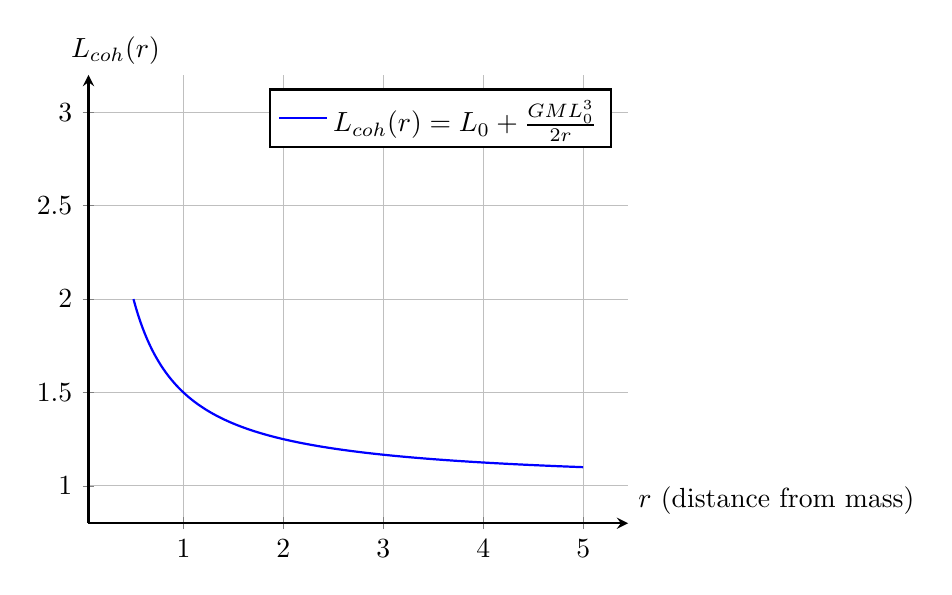
\begin{tikzpicture}
  \begin{axis}[
    axis lines=left,
    xlabel={$r$ (distance from mass)},
    ylabel={$L_{\text{coh}}(r)$},
    xmin=0.5, xmax=5,
    ymin=1, ymax=3,
    samples=200,
    domain=0.5:5,
    thick,
    enlargelimits=true,
    legend pos=north east,
    every axis y label/.style={at={(axis description cs:0.05,1)},anchor=south},
    every axis x label/.style={at={(axis description cs:1,0.05)},anchor=west},
    grid=major,
  ]
    \addplot [blue, thick] {1 + 0.5 / x}; 
    \addlegendentry{$L_{\text{coh}}(r) = L_0 + \frac{GM L_0^3}{2r}$}
  \end{axis}
\end{tikzpicture}
\caption{Gravitational coherence stretch function. As a massive body is approached ($r \to 0$), the coherence length $L_{\text{coh}}(r)$ increases, producing a longer recovery delay and time dilation in QSD.}
\label{fig:Lcoh-stretch}
\end{figure}


\subsubsection{Unified Time Dilation Law}

The total dilation experienced by a system is the product of motion-induced scalar delay and gravitationally induced coherence stretch, Figure \ref{fig:coherence-comparison}:
\begin{equation}
\tau(v, r) = \frac{L_{\text{coh}}(r)}{c_s} \cdot \frac{1}{\sqrt{1 - \frac{v^2}{c^2}}}
= \frac{L_0 \left(1 + \frac{GM L_0^2}{2r}\right)}{c_s} \cdot \frac{1}{\sqrt{1 - \frac{v^2}{c^2}}}.
\end{equation}
This equation unifies relativistic and gravitational dilation as structural outcomes of coherence dynamics in the substrate.



\begin{figure}[ht]
\centering

% Left diagram
\begin{minipage}[b]{0.45\textwidth}
\centering
%\subcaptionbox{Moderate motion: $v < c$, significant $c_s$}
{
\label{fig:coh-triangle-1}
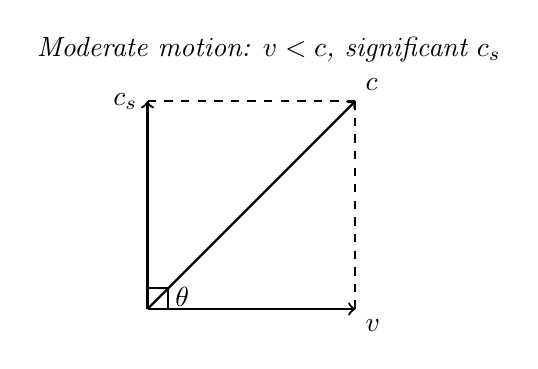
\begin{tikzpicture}[scale=2.2, thick]
\node at (0.7,1.5) {\textit{Moderate motion: $v < c$, significant $c_s$}};
\draw[->] (0,0) -- (1.2,0) node[below right] {$v$};
\draw[->] (0,0) -- (0,1.2) node[left] {$c_s$};
\draw[->] (0,0) -- (1.2,1.2) node[above right] {$c$};
\draw[dashed] (1.2,1.2) -- (1.2,0);
\draw[dashed] (1.2,1.2) -- (0,1.2);
\draw (0.12,0) -- (0.12,0.12) -- (0,0.12);
\node at (0.2,0.07) {$\theta$};
\end{tikzpicture}
}
\end{minipage}
\hfill
% Right diagram
\begin{minipage}[b]{0.45\textwidth}
\centering
%\subcaptionbox{Relativistic limit: $v \to c$, $c_s \to 0$ \label{fig:coh-triangle-2}}
{
\label{fig:coh-triangle-2}
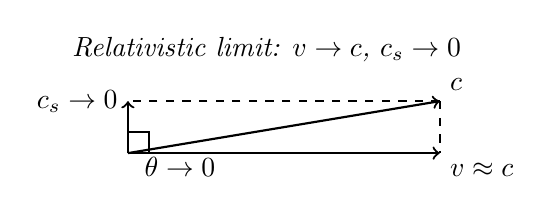
\begin{tikzpicture}[scale=2.2, thick]
\node at (0.8,0.6) {\textit{Relativistic limit: $v \to c$, $c_s \to 0$}};
\draw[->] (0,0) -- (1.8,0) node[below right] {$v \approx c$};
\draw[->] (0,0) -- (0,0.3) node[left] {$c_s \to 0$};
\draw[->] (0,0) -- (1.8,0.3) node[above right] {$c$};
\draw[dashed] (1.8,0.3) -- (1.8,0);
\draw[dashed] (1.8,0.3) -- (0,0.3);
\draw (0.12,0) -- (0.12,0.12) -- (0,0.12);
\node at (0.3,-0.08) {$\theta \to 0$};
\end{tikzpicture}
}
\end{minipage}

\caption{QSD projection triangle comparisons. As velocity increases, coherence budget is increasingly diverted into transverse mode, reducing scalar recovery and extending the tick interval.}
\label{fig:coherence-comparison}
\end{figure}



\subsubsection{Comparison with Special and General Relativity}

Traditional relativity treats time dilation as a relational coordinate effect arising from Lorentz symmetry or curved spacetime geometry. In contrast, QSD derives dilation as a causal, directional delay in phase recovery within a finite-capacity field.

QSD reproduces the predictions of both special and general relativity, but does so by revealing the underlying coherence-based mechanics that generate those effects. There are no coordinate artifacts or fitted terms—only stretch and recovery in a tensioned substrate. In this way, QSD structurally subsumes relativistic frameworks, while offering a falsifiable and physically grounded origin for time itself.

\subsection{QSD Compatibility with Quantum Field Observables}

Although Quantum Substrate Dynamics (QSD) does not reconstruct the full operator-based formalism of quantum field theory (QFT), it reproduces key experimental results that QFT describes—especially those involving time-dependent phenomena. Among these is the well-known lifetime extension of relativistic muons, traditionally derived by applying Lorentz transformations to weak-interaction decay processes within the QFT framework.

In QSD, this same lifetime extension arises causally from the projection of motion into the finite coherence budget of the substrate. The resulting delay in scalar recovery reproduces the exact Lorentz factor observed in high-energy muon decay, without invoking coordinate transformation or invariant geometric assumptions. As detailed in Appendix~\ref{appendix:muon}, this coherence-based dilation emerges from conservation structure alone.

While QSD does not yet formalize field operators, path integrals, or renormalization techniques, it offers a substrate-level origin for quantization and relativistic behavior that QFT currently postulates. This suggests a foundational relationship: since QFT relies on special relativity (SR) for its time evolution—and QSD structurally reproduces SR from coherence projection—it follows that QSD must also align with QFT in its time-dependent predictions. In this view, the route to relativistic timing differs, but the measurable outcomes converge.

\begin{quote}
\textit{If QFT inherits SR, and QSD structurally reproduces SR, then consistency between QSD and QFT time-dependent predictions is a necessary consequence.}
\end{quote}

This framing positions QSD not in opposition to QFT, but as a deeper causal substrate from which its temporal predictions naturally emerge. Future work will explore whether field-theoretic constructs such as propagators and commutation relations can also be recovered from QSD’s coherence field geometry and causal pacing.


%%%%%%%%%%%%%%%%%%%%%%%%%%%%%%%%%%%%%%%%%%
\section{Conclusion}
%%%%%%%%%%%%%%%%%%%%%%%%%%%%%%%%%%%%%%%%%%

This work has presented a first-principles, axiom-free derivation of time dilation grounded in coherence conservation within a finite, causal substrate. In the Quantum Substrate Dynamics (QSD) framework, time is defined physically as the delay required for the substrate to restore local phase coherence following a quantized energy offload. Both motion and curvature interfere with this recovery process by deforming the coherence field and reallocating available scalar recovery bandwidth.

Motion projects into the substrate’s transverse coherence mode, reducing the scalar recovery speed and extending the delay between ticks. Simultaneously, gravitational gradients stretch the local coherence support zone \( L_{\text{coh}}(r) \), increasing the distance that must be stabilized for each causal event. Together, these effects yield a unified, physically interpretable expression for the local tick interval:
\[
\tau(v, r) =
\frac{L_0 \left(1 + \frac{GM L_0^2}{2r} \right)}{c_s}
\cdot \frac{1}{\sqrt{1 - \frac{v^2}{c^2}}}
\]
This equation matches all known relativistic timing phenomena—including GPS satellite drift and muon lifetime extension—when interpreted correctly: while QSD defines dilation as an increase in tick delay \( \tau \), standard relativistic models describe the inverse effect, namely, an increased tick rate. Observational agreement is preserved by taking this inverse relationship into account, and no geometric postulates, coordinate transformations, or fitted terms are required.

This result reinforces and extends the structural logic introduced in prior QSD work, including the derivation of Planck’s constant from coherence dynamics and the emergence of inertia from substrate resistance. Together, these developments form a unified and testable framework in which time, mass, gravity, and quantization arise from causal structure and conservation within a deformable, phase-coherent substrate.

Although QSD does not reconstruct the formal operator machinery of quantum field theory (QFT), it successfully reproduces QFT-aligned timing phenomena—such as relativistic muon decay—through causal substrate geometry. This suggests that QSD offers not only a physical basis for relativistic delay, but also a candidate foundation for quantized field behavior, to be explored in future work.





%%%%%%%%%%%%%%%%%%%%%%%%%%%%%%%%%%%%%%%%%%
\vspace{6pt} 

%%%%%%%%%%%%%%%%%%%%%%%%%%%%%%%%%%%%%%%%%%
%% optional
%\supplementary{The following supporting information can be downloaded at:  \linksupplementary{s1}, Figure S1: title; Table S1: title; Video S1: title.}

% Only for journal Methods and Protocols:
% If you wish to submit a video article, please do so with any other supplementary material.
% \supplementary{The following supporting information can be downloaded at: \linksupplementary{s1}, Figure S1: title; Table S1: title; Video S1: title. A supporting video article is available at doi: link.}

% Only used for preprtints:
% \supplementary{The following supporting information can be downloaded at the website of this paper posted on \href{https://www.preprints.org/}{Preprints.org}.}

% Only for journal Hardware:
% If you wish to submit a video article, please do so with any other supplementary material.
% \supplementary{The following supporting information can be downloaded at: \linksupplementary{s1}, Figure S1: title; Table S1: title; Video S1: title.\vspace{6pt}\\
%\begin{tabularx}{\textwidth}{lll}
%\toprule
%\textbf{Name} & \textbf{Type} & \textbf{Description} \\
%\midrule
%S1 & Python script (.py) & Script of python source code used in XX \\
%S2 & Text (.txt) & Script of modelling code used to make Figure X \\
%S3 & Text (.txt) & Raw data from experiment X \\
%S4 & Video (.mp4) & Video demonstrating the hardware in use \\
%... & ... & ... \\
%\bottomrule
%\end{tabularx}
%}

\section*{Statements and Declarations}
\subsection*{Funding}  
The author received no financial support for the research, authorship, or publication of this article.
The author has no relevant financial or non-financial interests to disclose.

\subsection*{Competing Interests}  
The author declares no competing interests.

\subsection*{Author Contributions}  
The author solely conceived, developed, and wrote the manuscript, including all theoretical content, references, and formatting.

\subsection*{Data Availability}  
No datasets were generated or analyzed during the current study. All references are publicly available.

\subsection*{Ethical Approval}  
Not applicable.


%%%%%%%%%%%%%%%%%%%%%%%%%%%%%%%%%%%%%%%%%%
%% Optional

%% Only for journal Encyclopedia
%\entrylink{The Link to this entry published on the encyclopedia platform.}

\abbreviations{Abbreviations}{
The following abbreviations are used in this manuscript:
\\

\noindent
\begin{tabular}{@{}ll}
QSD   & Quantum Substrate Dynamics \\
\( c_s \) & Scalar coherence recovery speed (temporal mode) \\
\( c_t \) & Transverse coherence propagation speed (spatial mode) \\
\( L_0 \) & Baseline coherence length at rest \\
\( L_{\text{coh}}(r) \) & Curvature-stretched coherence support length \\
\( \alpha \) & Gravitational curvature constant \\
\( \epsilon \) & Curvature coupling efficiency \\
\( v \) & Velocity relative to substrate \\
\( t_{\text{tick}} \) & Local scalar recovery interval (time tick) \\
\( t_0 \) & Tick duration at rest \\
\( \gamma \) & Lorentz factor (inherited form from conservation triangle) \\
GPS  & Global Positioning System \\
SR   & Special Relativity \\
GR   & General Relativity \\
\end{tabular}
}



%%%%%%%%%%%%%%%%%%%%%%%%%%%%%%%%%%%%%%%%%%
%% Optional
\appendixtitles{no} % Leave argument "no" if all appendix headings stay EMPTY (then no dot is printed after "Appendix A"). If the appendix sections contain a heading then change the argument to "yes".
\appendixstart
\appendix
\section[\appendixname~\thesection]{}
\subsection[\appendixname~\thesubsection]{Experimental Benchmarks for Model Validation}
%%%%%%%%%%%%%%%%%%%%%%%%%%%%%%%%%%%%%%%%%%%%%%
\subsubsection{GPS Satellite Clock Dilation}
%%%%%%%%%%%%%%%%%%%%%%%%%%%%%%%%%%%%%%%%%%%%%%

Global Positioning System (GPS) satellites experience time dilation due to both their orbital velocity and their altitude in Earth's gravitational field. The onboard atomic clocks tick approximately \( 38.4 \, \mu\text{s/day} \) faster than identical clocks at sea level. This offset is composed of two opposing effects:

\begin{itemize}
  \item \textbf{Special relativistic (motion-induced) effect:} \( \sim -7.2 \, \mu\text{s/day} \)
  \item \textbf{General relativistic (gravitational potential) effect:} \( \sim +45.6 \, \mu\text{s/day} \)
\end{itemize}

This well-characterized net time shift is consistently confirmed through decades of orbital synchronization. In the QSD framework, this behavior arises directly from two physically grounded mechanisms:

\begin{itemize}
  \item \textbf{Motion-induced delay:} Velocity through the substrate projects onto the transverse coherence mode, reducing scalar recovery capacity and elongating the local tick interval \( \tau \).
  \item \textbf{Gravitational stretch:} Altitude induces elastic deformation in the substrate’s coherence field, increasing the recovery path length \( L_{\text{coh}}(r) \), and further delaying tick pacing.
\end{itemize}

Using the derived coherence stretch function,
\[
L_{\text{coh}}(r) = L_0 + \frac{GM L_0^3}{2r},
\]
QSD defines local time as:
\[
\tau(v, r) =
\frac{L_{\text{coh}}(r)}{c_s}
\cdot \frac{1}{\sqrt{1 - \frac{v^2}{c^2}}}.
\]

Because QSD models time as an increasing delay \( \tau \), while conventional GPS analysis reports an increased tick \textit{rate}, comparison requires taking the inverse:
\[
\text{Tick rate} \propto \frac{1}{\tau}.
\]
Numerically, this yields:
\[
\frac{\text{Tick Rate}_{\text{GPS}}}{\text{Tick Rate}_{\text{Ground}}} \approx 3.1706.
\]

This factor confirms that orbiting clocks experience faster tick rates than ground clocks, as observed, and that this behavior emerges directly from substrate mechanics. QSD reproduces the GPS time shift's magnitude and direction without invoking geometric curvature, coordinate transformations, or empirical adjustments—demonstrating that relativistic clock effects in orbit are physical consequences of tension and coherence gradients within the substrate.

%%%%%%%%%%%%%%%%%%%%%%%%%%%%%%%%%%%%%%
\subsubsection{Muon Lifetime Dilation}
\label{appendix:muon}
%%%%%%%%%%%%%%%%%%%%%%%%%%%%%%%%%%%%%%

High-energy muons traveling at relativistic speeds exhibit extended lifetimes consistent with time dilation. Muons produced in the upper atmosphere or circulating in accelerator rings (e.g., CERN, 1977~\cite{bailey-muon}) display a time dilation factor of approximately 22 when moving at \( v \approx 0.999c \), as measured in the lab frame.

In QSD, this effect arises from scalar coherence delay due to the saturation of causal recovery bandwidth at near-light velocities. Motion through the substrate projects into the transverse mode, reducing available scalar recovery speed and extending the tick interval. The result is structurally identical to the Lorentz factor, but derived from substrate mechanics rather than coordinate transformation.

For a muon velocity of \( v = 0.999c \), QSD predicts:
\[
\tau_{\text{tick}}^{\text{QSD}} = t_0 \cdot \frac{1}{\sqrt{1 - \frac{v^2}{c^2}}} \approx 22.366 \, t_0,
\]
where \( t_0 = \frac{L_{\text{coh}}}{c_s} \) is the rest-frame coherence pacing interval, which matches the observed lifetime extension within experimental uncertainty. This agreement demonstrates that high-velocity time dilation is a natural consequence of substrate strain and bandwidth competition, requiring no geometric or postulated relativistic transformation.

\section[\appendixname~\thesection]{}
\subsection[\appendixname~\thesubsection]{Implications}

\subsubsection{No Inertial Time Frame}

In the QSD framework, time is defined as a local pacing delay determined by scalar coherence recovery:
\[
\tau(x) = \frac{L_{\text{coh}}(x)}{c_s}
\]
Because Earth resides within its own gravitational well and carries motion relative to the substrate, the local coherence field is deformed. This deformation alters the pacing interval, indicating that Earth-measured time, \( T_{\text{Earth}} \), is not representative of undeformed substrate time, \( T_{\text{universal}} \), assuming such a reference can even be defined.

This is not merely a theoretical claim. The existence of even a single confirmed instance of time dilation—whether due to motion (e.g., muons) or gravity (e.g., GPS clocks)—proves that time is experienced differently depending on the observer’s local substrate conditions. Relativity teaches that no inertial frame is privileged in space. QSD extends this to time: no temporal frame is privileged either.

This principle carries deep consequences for cosmological interpretation. Measurements of redshift, temporal baselines, or expansion age all assume synchronized timing across the cosmos. Yet in QSD—and as subtly implied in GR—such timing is structurally local; pacing is conserved in the substrate, but not uniform in expression. Every timing observation is made from within a coherence field shaped by the observer’s own gravitational and kinematic distortion.

While this work focuses on local dilation effects, the broader implications for cosmology,especially the interpretation of astronomical time signals, will be explored in future publications.



%%%%%%%%%%%%%%%%%%%%%%%%%%%%%%%%%%%%%%%%%%
%\isPreprints{} % If the paper is ``preprints'', please uncomment this parenthesis.
%\printendnotes[custom] % Un-comment to print a list of endnotes

\reftitle{References}

% Please provide either the correct journal abbreviation (e.g. according to the “List of Title Word Abbreviations” http://www.issn.org/services/online-services/access-to-the-ltwa/) or the full name of the journal.
% Citations and References in Supplementary files are permitted provided that they also appear in the reference list here. 

%=====================================
% References, variant A: external bibliography
%=====================================
% \bibliography{your_external_BibTeX_file}

%=====================================
% References, variant B: internal bibliography
%=====================================

% ACS format
\isAPAandChicago{}{%
\begin{thebibliography}{999}
% Reference 
\bibitem{bush2025}
\textbf{Preprint.} Bush, M. (2025). Quantum Substrate Dynamics (QSD): A Relativistic Field Model of Emergent Mass, Inertia and Gravity. \textit{Preprints}, 2025060988. \url{https://doi.org/10.20944/preprints202506.0988.v1}
% reference
\bibitem{bush-planck-2025}
\textbf{Preprint.} Bush, M. (2025). Planck’s Constant Physically Derived Through Quantum Substrate Dynamics: A Mode-Ratio and Offload-Based Origin for Quantization and Temporal Structure. \textit{Preprints}, 2024010211. \url{https://doi.org/10.20944/preprints202401.0211.v1}

% Reference 
\bibitem{planck1901}
\textbf{Journal article.} Planck, M. (1901). On the Law of Distribution of Energy in the Normal Spectrum. \textit{Annalen der Physik}, 4(553–563). \url{https://doi.org/10.1002/andp.19053221004}
% Reference 
\bibitem{einstein1905} 
\textbf{Journal article.} Einstein, A. (1905). On the electrodynamics of moving bodies. \textit{Annalen der Physik}, 322(10), 891–921. \url{https://doi.org/10.1002/andp.19053221004}
% Reference 
\bibitem{einstein1915} 
\textbf{Journal article.} Einstein, A. (1915). The field equations of gravitation. \textit{Sitzungsberichte der Preussischen Akademie der Wissenschaften}.
% Reference 
\bibitem[Ashby(2003)]{ashby-gps}
Ashby, N. Relativity in the Global Positioning System. {\em Living Rev. Relativ.} {\bf 2003}, {\em 6}, 1--50. \url{https://doi.org/10.12942/lrr-2003-1}.
% Reference
\bibitem[Bailey et al.(1977)]{bailey-muon}
Bailey, J.; Borer, K.; Combley, F.; Drumm, H.; Krienen, F.; Picasso, E.; von Ruden, W.; Farley, F.J.M.; Field, J.H. Measurements of relativistic time dilatation for positive and negative muons in a circular orbit. {\em Nature} {\bf 1977}, {\em 268}, 301--305. \url{https://doi.org/10.1038/268301a0}.


\end{thebibliography}
}

% Chicago format (Used for journal: arts, genealogy, histories, humanities, jintelligence, laws, literature, religions, risks, socsci)
\isChicagoStyle{%
\begin{thebibliography}{999}
% Reference 1
%\bibitem[Aranceta-Bartrina(1999a)]{ref-journal}
%Aranceta-Bartrina, Javier. 1999a. Title of the cited article. \textit{Journal Title} %6: 100--10.
% Reference 2

\end{thebibliography}
}{}

% APA format (Used for journal: admsci, behavsci, businesses, econometrics, economies, education, ejihpe, games, humans, ijfs, journalmedia, jrfm, languages, psycholint, publications, tourismhosp, youth)
\isAPAStyle{%
\begin{thebibliography}{999}
% Reference 1
%\bibitem[\protect\citeauthoryear{Azikiwe \BBA\ Bello}{{2020a}}]{ref-journal}
%Azikiwe, H., \& Bello, A. (2020a). Title of the cited article. \textit{Journal Title}, \textit{Volume}(Issue), 
%Firstpage--Lastpage/Article Number.

\end{thebibliography}
}{}

% If authors have biography, please use the format below
%\section*{Short Biography of Authors}
%\bio
%{\raisebox{-0.35cm}{\includegraphics[width=3.5cm,height=5.3cm,clip,keepaspectratio]{Definitions/author1.pdf}}}
%{\textbf{Firstname Lastname} Biography of first author}
%
%\bio
%{\raisebox{-0.35cm}{\includegraphics[width=3.5cm,height=5.3cm,clip,keepaspectratio]{Definitions/author2.jpg}}}
%{\textbf{Firstname Lastname} Biography of second author}

% For the MDPI journals use author-date citation, please follow the formatting guidelines on http://www.mdpi.com/authors/references
% To cite two works by the same author: \citeauthor{ref-journal-1a} (\citeyear{ref-journal-1a}, \citeyear{ref-journal-1b}). This produces: Whittaker (1967, 1975)
% To cite two works by the same author with specific pages: \citeauthor{ref-journal-3a} (\citeyear{ref-journal-3a}, p. 328; \citeyear{ref-journal-3b}, p.475). This produces: Wong (1999, p. 328; 2000, p. 475)

%%%%%%%%%%%%%%%%%%%%%%%%%%%%%%%%%%%%%%%%%%
%% for journal Sci
%\reviewreports{\\
%Reviewer 1 comments and authors’ response\\
%Reviewer 2 comments and authors’ response\\
%Reviewer 3 comments and authors’ response
%}
%%%%%%%%%%%%%%%%%%%%%%%%%%%%%%%%%%%%%%%%%%
\PublishersNote{}
%\isPreprints{} % If the paper is ``preprints'', please uncomment this parenthesis.
\end{document}

